\documentclass[conference]{IEEEtran}
% *** GRAPHICS RELATED PACKAGES ***
%
\ifCLASSINFOpdf
  \usepackage[pdftex]{graphicx}
  % declare the path(s) where your graphic files are
  % \graphicspath{{../pdf/}{../jpeg/}}
  % and their extensions so you won't have to specify these with
  % every instance of \includegraphics
  \DeclareGraphicsExtensions{.pdf,.jpeg,.png}
\else
  % or other class option (dvipsone, dvipdf, if not using dvips). graphicx
  % will default to the driver specified in the system graphics.cfg if no
  % driver is specified.
  \usepackage[dvips]{graphicx}
  % declare the path(s) where your graphic files are
  % \graphicspath{{../eps/}}
  % and their extensions so you won't have to specify these with
  % every instance of \includegraphics
  % \DeclareGraphicsExtensions{.eps}
\fi

\usepackage{pgf}
%\usepackage{tikz}
%\usetikzlibrary{arrows,automata}

\definecolor{darkgreen}{rgb}{0,0.7,0}

\newif\ifdraft
\drafttrue
%\draftfalse
\ifdraft
 \newcommand{\katznote}[1]{ {\textcolor{blue} { ***Dan:   #1 }}}
 \newcommand{\ketanote}[1]{{\textcolor{orange}  { ***Ketan:   #1 }}}
 \newcommand{\kriedernote}[1]{ {\textcolor{darkgreen}  { ***Scott:   #1 }}}
 \newcommand{\note}[1]{ {\textcolor{red}    {\bf #1 }}}
\else
 \newcommand{\katznote}[1]{}
 \newcommand{\kriedernote}[1]{}
 \newcommand{\note}[1]{}
\fi
% correct bad hyphenation here
%\hyphenation{op-tical net-works semi-conduc-tor}

\hyphenation{Queuing}

\begin{document}
%
% can use linebreaks \\ within to get better formatting as desired
\title{Accelerating Scientific Workflow Applications with GPUs}

%\author{\IEEEauthorblockN{Auth1\IEEEauthorrefmark{1},
%Auth2\IEEEauthorrefmark{1}\IEEEauthorrefmark{1}, 
%Auth3\IEEEauthorrefmark{1},
%\IEEEauthorblockA{\IEEEauthorrefmark{1}Argonne National Laboratory}
%}}

\author{Dustin Shahidehpour\IEEEauthorrefmark{1},
Scott J. Krieder\IEEEauthorrefmark{1},
Jeffrey Johnson\IEEEauthorrefmark{1}\\
Benjamin Grimmer\IEEEauthorrefmark{1},
Justin M. Wozniak\IEEEauthorrefmark{2},
Michael Wilde\IEEEauthorrefmark{2}\IEEEauthorrefmark{3},
Ioan Raicu\IEEEauthorrefmark{1}\IEEEauthorrefmark{2}\\
\IEEEauthorblockA{
\IEEEauthorrefmark{1}Department of Computer Science, Illinois Institute of Technology}
\IEEEauthorrefmark{2}MCS Division, Argonne National Laboratory\\
\IEEEauthorrefmark{3}Computation Institute, University of Chicago
}


\maketitle


\begin{abstract}
This work analyzes the performance increases gained from enabling SwiH applications to utilize the GPU through the GeMTC Framework. By identifying computationally intensive portions of SwiH applications, we can easily turn these code blocks into GeMTC microkernels. Users can then call these microkernels throughout the lifetime of their SwiH application. The GeMTC API handles task overlap and data movement, providing transparent GPU acceleration for the user. This work highlights preliminary performance results from the scientific application MDProxy. This application determines the energy of particles in a modeled universe as they move around in space.
\end{abstract}

% no keywords
\begin{IEEEkeywords}
Many-Task Computing, Swift, GPGPU, CUDA
\end{IEEEkeywords}

\IEEEpeerreviewmaketitle

\section{Background Information}
GeMTC (GPU enabled Many-Task Computing), is a CUDA-based framework which provides efficient support for Many-Task Computing workloads on accelerators. The GeMTC framework has been integrated into SwiH/T, a parallel programming framework from Argonne National Laboratory and the University of Chicago, providing GPU functionality for the Swift language.

A microkernel is a traditional CUDA kernel that is modified to run in the GeMTC framework. A CUDA kernel is a user-defined function that runs on a NVIDIA GPU.

\section{MDProxy Architecture}

\section{MDProxy Evaluation}

\section{Hardware Enironment}

\section{Conclusions}

\section{Future Work}

\section{Introduction}
This work aims to provide an integration between data-flow driven parallel programming systems (e.g. Many-Task Computing - MTC) and hardware accelerators \cite{kriederGCASR12} (e.g. NVIDIA GPUs, AMD GPUs, and the Intel MIC). MTC aims to bridge the gap between two computing paradigms, high throughput computing (HTC) and high-performance computing (HPC). MTC emphasizes using many computing resources over short periods of time to accomplish many computational tasks (i.e. including both dependent and independent tasks), where the primary metrics are measured in seconds.\cite{raicu2008toward} Swift is a particular implementation of the MTC paradigm, and is a parallel programming system that has been successfully used in many large-scale computing applications. \cite{zhao2007swift} The scientific community has adopted Swift as a great way to increase productivity in running complex applications via a dataflow driven programming model, which intrinsically allows implicit parallelism to be harnessed based on data access patterns and dependencies. Swift is a parallel programming system that fits the MTC model, and has been shown to run well on tens of thousands of nodes with task graphs in the range of hundreds of thousands of tasks. This work aims to enable Swift to efficiently use accelerators (such as NVIDIA GPUs and Intel MIC) to further accelerate a wide range of applications, on a growing portion of high-end systems.

\section{GeMTC}

Currently CUDA developers may only have a maximum of 16 kernels running concurrently, one kernel per streaming multiprocessor (SM). The problem is that all kernels have to start and end at the same time, causing extreme inefficiencies in heterogeneous workloads. By working at the warp level we trade local memory for concurrency and we are able to run up to 84 concurrent kernels. \cite{kriederSC12} This middleware allow independent kernels (MIMD style) to be launched and managed on many-core architectures that traditionally only support SIMD. \cite{kriederXSEDE12} In Figure \ref{fig:big_pic} Swift/T is calling the GeMTC API and passing tasks into memory on the device. Warp workers pick up those tasks, execute with the given parameters and place results on an outgoing result queue. This execution model is shown in further detail in Figure \ref{fig:warps}. Finally, Swift/T will poll the device return results from the result queue back to the appropriate task in the swift script. Figure \ref{fig:block_diagram} is a  GK110 block diagram as presented by NVIDIA. \cite{GK110} This diagram demonstrates how the current generation GPUs have O(10) Streaming Multiprocessors (SMX), O(100) Warps, and O(1000) cores.
\begin{figure}[h]
\centering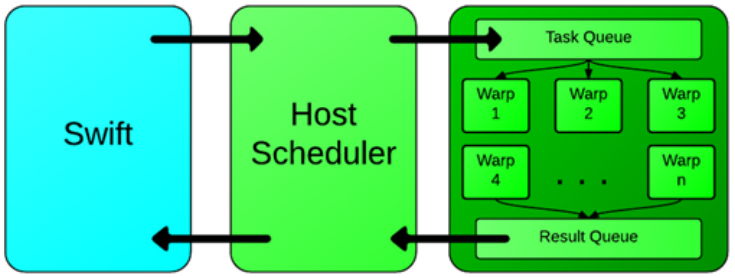
\includegraphics[width=8cm]{imgs/big_picture.png}
\caption{Flow of a task through Swift/T and GeMTC.}
\label{fig:big_pic}
\end{figure}

\begin{figure}[h]
\centering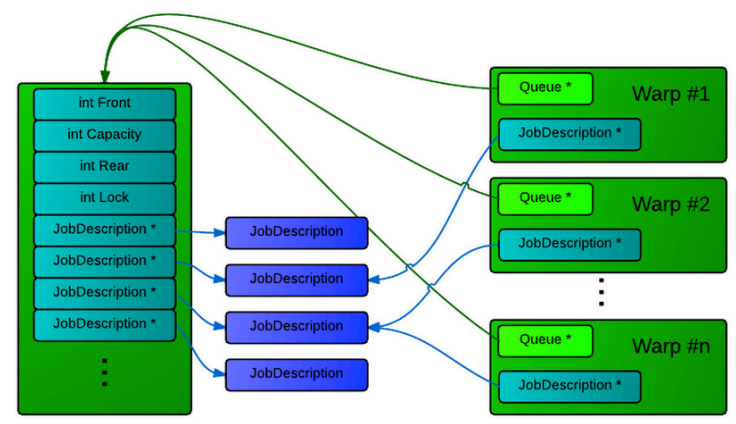
\includegraphics[width=8cm]{imgs/warps.png}
\caption{Worker interaction with incoming work queue.}
\label{fig:warps}
\end{figure}

\begin{figure}[h]
\centering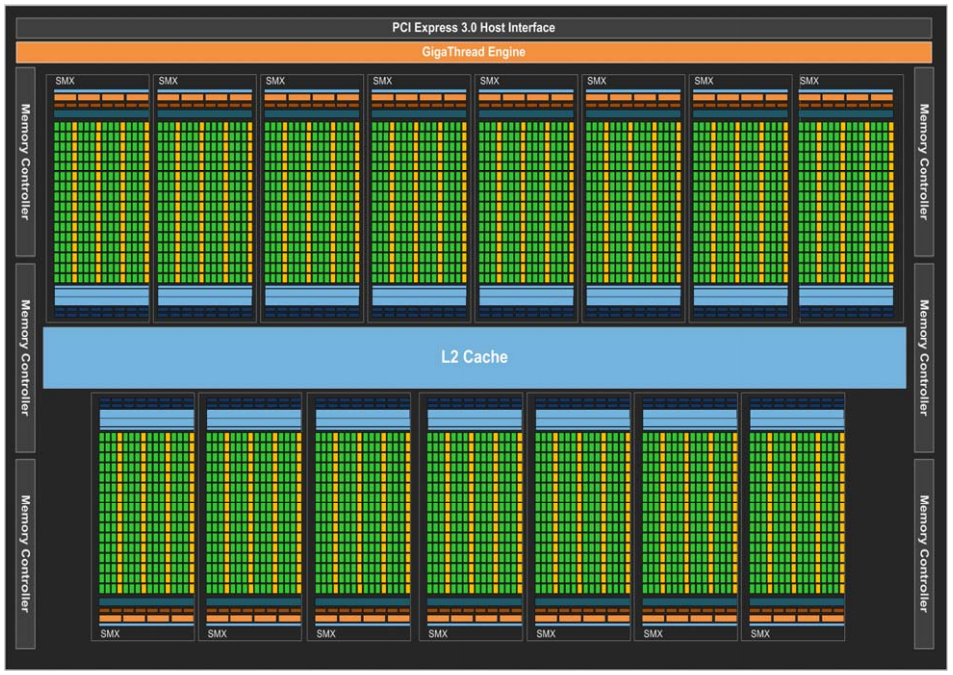
\includegraphics[width=8cm]{imgs/blockdiagram.png}
\caption{Kepler GK110 full chip block diagram.}
\label{fig:block_diagram}
\end{figure}

\section{Swift/T}
Swift is an implicitly parallel scripting language. By operating on data-flow driven scheduling of parallel tasks Swift is capable of extracting parallelism out of an application. The distributed executor eliminates centralized bottlenecks and an optimized compiler detects errors ahead of runtime for improved efficiency. Swift has been shown to scale over 100k cores and is portable to most MPI-based clusters. Finally, it's familiar C/Java like syntax makes it easy for developers to quickly understand language constructs. The diagram in Figure \ref{fig:swiftt} demonstrates the 4 portions of the Swift stack which contains (1)A high level Swift Script, (2)A compiler, namely STC, to generate (3)An intermediate code and (4)Execution of the intermediate code. The most recent version of Swift, namely Swift/T, supports function calls.\cite{wozniak13swift} This work also presents a novel API to allow interaction between GeMTC and Swift/T. By integrating the GeMTC middleware into the Swift/T stack Swift is capable of calling C wrapper functions to CUDA kernels/applications directly. 

\begin{figure}[h]
\centering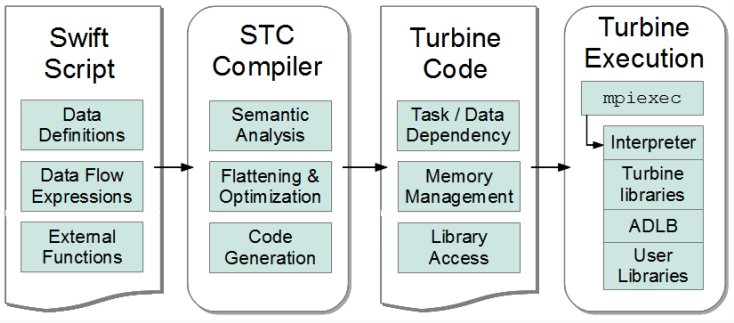
\includegraphics[width=8cm]{imgs/swiftt.png}
\caption{Overview of the Swift/T tool chain.}
\label{fig:swiftt}
\end{figure}



\section{Preliminary Results}
In this section we present preliminary results from the integration of GeMTC and Swift/T. In Figure \ref{fig:multinode} we demonstrate the efficiency of Swift/T and GeMTC on 4 Cray XK7 nodes. Swift/T is launching 50k system wide tasks for which there are known completion times. Efficiency is set to actual run time / expected runtime. Evaluation takes place on 1 to 4 nodes of Cray XK7 machines with 156 GPU workers (the maximum) on each NVIDIA K20 GPU. Tasks lasting longer that 400ms are shown to have good efficiency and at 4-node scale we are capable of maintaining 4k tasks per second system wide.
%\begin{figure}[h]
%\centering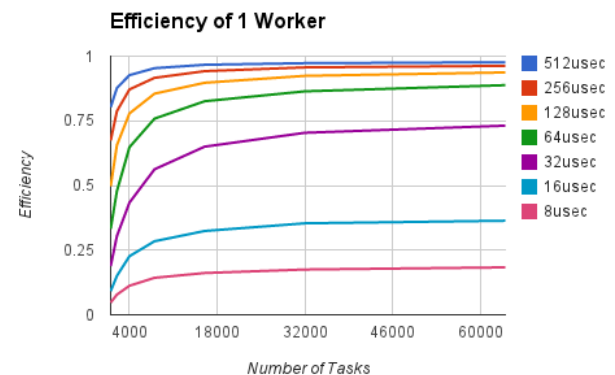
\includegraphics[width=8cm]{imgs/1worker.png}
%\caption{GeMTC efficiency from launching a single worker on the GPU.}
%\label{fig:1worker}
%\end{figure}

%\begin{figure}[h]
%\centering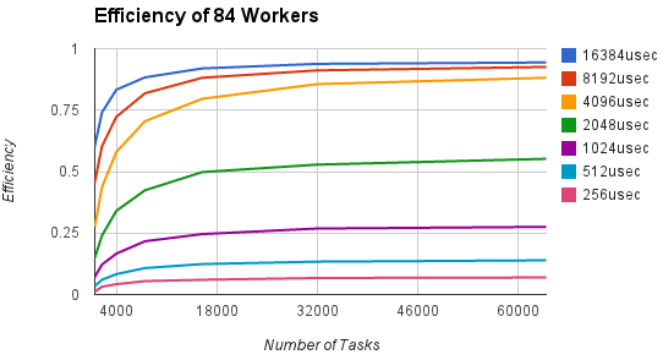
\includegraphics[width=8cm]{imgs/84workers.png}
%\caption{GeMTC efficiency launching maximum workers on GTX680.}
%\label{fig:84workers}
%\end{figure}

\begin{figure}[h]
\centering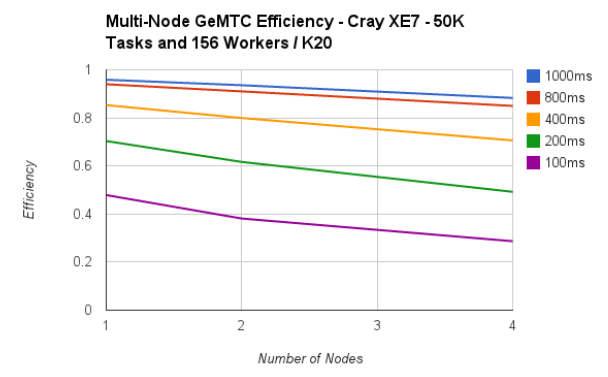
\includegraphics[width=8cm]{imgs/multinode.png}
\caption{GeMTC + Swift/T efficiency on 4 XK7 nodes.}
\label{fig:multinode}
\end{figure}

%\begin{figure}[h]
%\centering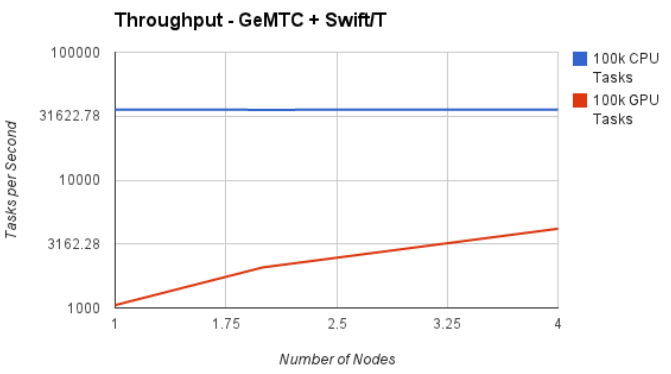
\includegraphics[width=8cm]{imgs/throughput4nodes.png}
%\caption{GeMTC + Swift/T throughput on 4 XK7 nodes.}
%\label{fig:throughput}
%\end{figure}

\section{Conclusions and Future Work}
In this work we designed and implemented the GeMTC framework. A sub-allocator provides improved memory management for dynamic tasks. Integration between GeMTC + Swift/T provides application support, data-flow parallelism, and multi-node scalability. Finally, we evaluated synthetic benchmarks and demonstrated improved performance. Future work aims to abstract for additional accelerator support, evaluate real applications such as the Open Protein Simulator (OOPS) \cite{OOPS}, and improve current framework performance.

\bibliographystyle{IEEEtran}
\bibliography{ref}
\end{document}
